In the following, SLIM is used in different configurations as a surrogate for modelling the benefit present values of two insurance tariffs. The results are interpreted and the fidelity is compared with the MBT algorithms GUIDE, MOB and CTree.

\subsection{Data set K2204}
The data set K2204 contains data for a (fictitious) endowment insurance tariff and includes the features sex, age and duration and the two targets benefit present value (BPV) and premium present value (PPV). The targets were modelled using two different black box models.  
In the following, only the BPV is considered. The results for the PBV are very similar (interpreted the other way round) and can be found in the appendix. A special characteristic of this data set is a correlation between the Age and Duration features, as can be seen in Figure \ref{fig:ins_corr_age_duration}. When interpreting the MBT, it must therefore be taken into account that a split with regard to one of the features always has an influence on the value range of the other feature.

\begin{figure}[!htb]
    \centering    
    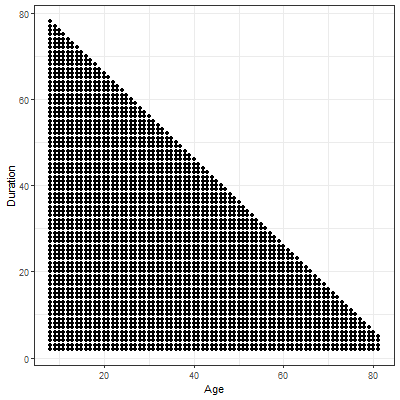
\includegraphics[width=7cm]{Figures/insurance_use_case/k2204_BPV/corr_age_duration.png}
    \caption{Features Age and Duration in the K2204 data set}
    \label{fig:ins_corr_age_duration}
\end{figure}

In a first step, SLIM was fitted with linear regression models in the nodes. The maximum depth was set to 3 and an improvement in the objective of at least 0.1 of the previous improvement was set as prepruning parameter.
 The resulting tree is shown in Figure \ref{fig:ins_slim_lm_tree}.

 \begin{figure}[!htb]
     \centering     
     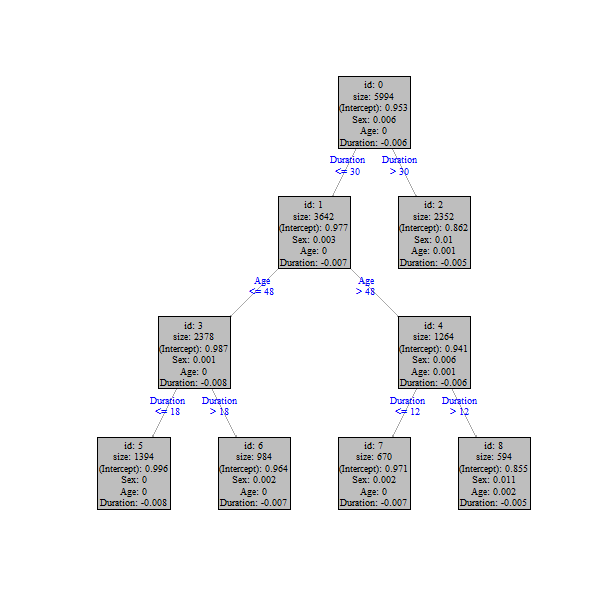
\includegraphics[width = 16cm]{Figures/insurance_use_case/k2204_BPV/slim_lm_tree.png}
     \caption{SLIM tree for K2204 with linear models}
     \label{fig:ins_slim_lm_tree}
 \end{figure}
 
\subsection{Data set R108}